% TODO introduire l'application, les fonctionnalités et les types d'user brièvement

\chapter{Analyse des besoins}
\label{chapter:analyseDesBesoins}
% Partie dans laquelle on explique les features / requirements attendues
% On y trouve sans doute :

\epigraph{<< Les choses paraissent simples jusqu'à ce qu'on commence à les analyser >>}{Audrey Niffenegger}

La phase d'analyse est dans la vie d'un projet l'une des phases les plus critiques, car celle-ci formalise les besoins des clients sous tous ses aspects afin que toutes les parties (dont les développeurs) puissent se mettre d'accord. Pour pallier les nombreuses difficultés inhérentes au contexte, plusieurs méthodes reconnues existent (notamment \Gls{QQOQCCP} et UML). \\

La principale fonctionnalité attendue de l'application web est la recherche de \glspl{fiche} sur base d'une combinaison de critères divers et variés (dont notamment des \glspl{tag}) pourrait sembler à première vue simple, mais il n'en est rien. En effet, la question sous-jacente est le problème du référencement de \glspl{resinfo}. Contrairement à d'autres domaines et l'existence de normes pour organiser les informations d'une \gls{resinfo} (\textit{Dublin Core} / \textit{LOM} pour ne citer que quelques unes), il n'existe pas de consensus sur l'arborescence / la taxonomie des \glspl{tag} (cf annexe \ref{annexe:AnalyseBiblio}).

\section{Analyse fonctionnelle}
\label{section:analyseFonctionnelle}

\subsection*{Les différents types d'utilisateurs}

% Comme expliqué par les Echos\cite{SOD}, la séparation des tâches est "un concept qui requière différents acteurs possédant des rôles et responsabilités différents pour la réalisation d’un ensemble de tâches dont l’exécution par un unique acteur pourrait potentiellement conduire à des fraudes ou des erreurs". \\


\paragraph{} \texttt{SourceCode} repose sur la participation active d'acteurs variés. Cela nécessite la mise en place d'une organisation sous forme de rôles afin de maintenir cette plateforme de ressources \textit{cohérente} et \textit{qualitative}. Notre analyse nous a permis d'isoler \textbf{4 types d'utilisateurs} disposant de \textit{privilèges additionnels} (en plus de leurs privilèges propres, chacun hérite aussi de ceux du précédent de la présente liste) :

\begin{itemize}
    \item \textbf{Visiteur} : Il s'agit d'un utilisateur non inscrit à notre plateforme. Il ne peut rechercher et consulter que les \glspl{fiche} de ressources validées par un administrateur.
    \item \textbf{Utilisateur} : Il s'agit d'un utilisateur  inscrit à notre plateforme. Celui-ci peut proposer de nouvelles ressources et maintenir les \glspl{fiche} dont il est le créateur.
    \item \textbf{Administrateur} : Celui-ci crée/modifie des ressources de toute nature (\glspl{fiche} proposées par les utilisateurs, \glspl{tag} et \glspl{tagCat}), en plus de classifier les \glspl{fiche}.
    \item \textbf{Super Administrateur} : Celui-ci dispose du droit de supprimer de manière définitive les différentes ressources de notre plateforme (y compris les \glspl{tag} et \glspl{tagCat}).
\end{itemize}

\subsection*{Fonctionnalités}

Pour réaliser les défis expliqués à la section \ref{section:challengesToDefeat}, il convient de faire l'inventaire des nombreuses fonctionnalités à réaliser de manière formelle.
Afin de les prioriser en fonction de leurs importances respectives, nous avons utilisé la méthode \textit{\textbf{M}o\textbf{S}\textbf{C}o\textbf{W}}\cite{MoSCoW}. Celle-ci consiste à classifier chaque tâche sous l'une des 4 lettres en gras qui composent cet acronyme en anglais dont voici la signification pour chacune :
\begin{itemize}
    \item \textcolor{red}{\textbf{M}ust} : C'est ce qui "doit être fait" (\textbf{vital})
    \item \textcolor{orange}{\textbf{S}hould} : C'est ce qui "devrait être fait dans la mesure du possible" (\textbf{essentiel})
    \item \textcolor{green}{\textbf{C}ould} : C'est ce qui "pourrait être fait dans la mesure où cela n'a pas d'impact sur les autres tâches" (\textbf{confort})
    \item \textcolor{gray}{\textbf{W}on't} : C'est ce qui "ne sera pas fait cette fois, mais sera fait plus tard" (\textbf{luxe})
\end{itemize}

À titre informatif, le choix du \textbf{JSON} se justifie par la norme que nous avons élaborée (cf annexe \ref{annexe:AnalyseBiblio}), qui l'utilise afin de pouvoir manipuler plus aisément les données contenues dans celui-ci.
Des explications complémentaires sur d'autres aspects de cet inventaire seront apportées dans les prochaines sections de ce chapitre.

\subsubsection*{Tout visiteur peut : }

\begin{itemize}
    \item[\textcolor{red}{\textbf{M}}] Rechercher des \glspl{fiche} dans l'application. La recherche se porte sur une combinaison libre des critères suivants : 
    \begin{itemize}
        \item[\textcolor{red}{\textbf{M}}] Rechercher dans les \glspl{tag} des \glspl{fiche}
        \item[\textcolor{red}{\textbf{M}}] Rechercher dans le titre des \glspl{fiche}
        \item[\textcolor{red}{\textbf{M}}] Rechercher les \glspl{fiche} par leurs états
        \item[\textcolor{red}{\textbf{M}}] Rechercher les \glspl{fiche} sur base d'un certain seuil sur le résultat moyen accordé par les utilisateurs
        \item[\textcolor{red}{\textbf{M}}] Rechercher les \glspl{fiche} par leurs créateurs
        \item[\textcolor{red}{\textbf{M}}] Rechercher les \glspl{fiche} par leurs identifiants
    \end{itemize}
        \item[\textcolor{red}{\textbf{M}}] Consulter une \gls{fiche}
    \item[\textcolor{red}{\textbf{M}}] Consulter les \glspl{tag} et \glspl{tagCat} existants (optionnellement avec des statistiques d'utilisation de ceux-ci)
    \item[\textcolor{red}{\textbf{M}}] S'inscrire à l'application
    \item[\textcolor{red}{\textbf{M}}] Se connecter à l'application via une adresse mail et un mot de passe
    \item[\textcolor{orange}{\textbf{S}}] Ordonner les \glspl{fiche} lors de la recherche avec une libre combinaison des paramètres suivants (en précisant pour chacun l'ordre du tri : ascendant / descendant) :
            \begin{itemize}
            \item le résultat moyen des votants pour une \gls{fiche}
            \item le nombre de votants pour une \gls{fiche}
            \item la date de la dernière modification de la \gls{fiche}
            \item le titre de la \gls{fiche}
            \item l'état de la \gls{fiche}
            \item l'identifiant de la \gls{fiche}
        \end{itemize}
    \item[\textcolor{green}{\textbf{C}}] Choisir quelles propriétés des \glspl{fiche} que l'on souhaite consulter
    \item[\textcolor{green}{\textbf{C}}] Télécharger la source d'une \gls{fiche} 
\end{itemize}

\subsubsection*{Tout utilisateur peut : }
\begin{itemize}
    \item[\textcolor{red}{\textbf{M}}] Mettre en ligne une \gls{fiche}  (avec éventuellement un fichier)
    \item[\textcolor{red}{\textbf{M}}] Modifier les informations d'une \gls{fiche}  lui appartenant
    \item[\textcolor{red}{\textbf{M}}] Changer l'état d'une \gls{fiche} lui appartenant (des restrictions que nous détaillerons dans la section TODO sont présentes pour éviter des dérives)
    \item[\textcolor{red}{\textbf{M}}] Proposer un nouveau ou plusieurs mot(s) clé(s)
    \item[\textcolor{orange}{\textbf{S}}] Gérer des favoris
    \item[\textcolor{orange}{\textbf{S}}] Utiliser des favoris dans la recherche de \gls{fiche}s
    \item[\textcolor{orange}{\textbf{S}}] Évaluer une \gls{fiche}  
    \item[\textcolor{orange}{\textbf{S}}] Consulter / Modifier ses informations personnelles
\end{itemize}

\subsubsection*{Tout administrateur peut : }
\begin{itemize}
    \item[\textcolor{red}{\textbf{M}}] Importer plusieurs \glspl{fiche} sur base d'un fichier JSON.
        Cette fonctionnalité comprend les fonctionnalités sous-jacentes suivantes :
        \begin{itemize}
            \item Ajouter éventuellement un état spécifique pour chacune des \glspl{fiche} à importer
            \item Créer automatiquement les \glspl{tag} non existants dans le système (avec éventuellement un état de départ)
            \item Créer automatiquement les \glspl{tagCat} non existantes dans le système
            \item Associer les \glspl{tag} à leurs \glspl{fiche} respectives. 
        \end{itemize}
    \item[\textcolor{red}{\textbf{M}}] Exporter des \glspl{fiche} au format JSON
    \item[\textcolor{red}{\textbf{M}}] Proposer un nouveau ou plusieurs mot(s) clé(s) (avec éventuellement un état spécifique pour chacun)
    \item[\textcolor{red}{\textbf{M}}] Modifier un \gls{tag} 
    \item[\textcolor{red}{\textbf{M}}] Modifier une \gls{tagCat} 
    \item[\textcolor{red}{\textbf{M}}] Changer l'état d'un ou plusieurs mot(s) clé(s)
    \item[\textcolor{red}{\textbf{M}}] Modifier les informations d'une \gls{fiche} 
    \item[\textcolor{red}{\textbf{M}}] Changer l'état d'une \gls{fiche} (aucune restriction)
    \item[\textcolor{red}{\textbf{M}}] Créer ou trouver des \glspl{tagCat}
    \item[\textcolor{orange}{\textbf{S}}] Lister tous les utilisateurs de l'application (sans distinction)
\end{itemize}

\subsubsection*{Tout super administrateur peut : }
\begin{itemize}
    \item[\textcolor{red}{\textbf{M}}] Supprimer des \glspl{fiche} / \glspl{tag} / \glspl{tagCat}
    \item[\textcolor{orange}{\textbf{S}}] Modifier le type d'un utilisateur
    \item[\textcolor{gray}{\textbf{W}}] Créer de nouveaux utilisateurs
\end{itemize}
\pagebreak

\subsection*{Recherche par \glspl{tag}}

Une interrogation légitime est de savoir comment exprimer la recherche par \glspl{tag}, ce qui n'est bien entendu pas chose aisée.
Pour l'illustrer, prenons l'exemple de quelques \glspl{fiche} et \glspl{tag}, que nous noterons resp. \textit{F}\textbf{X} et \textit{M}\textbf{X}
(\textbf{X} étant remplacé par un numéro pour les distinguer), avec quelques exemples de requêtes.

\begin{table}[H]
    \centering
    \begin{tabular}{|c|c|c|c|}
        \hline
            & M1 & M2 & M3 \\ \hline
            F1 & X  & X  &    \\ \hline
            F2 &    & X  & X  \\ \hline
            F3 & X  &    &    \\ \hline
    \end{tabular}
    \caption{Problématique de la recherche par \glspl{tag}}
    \label{tab:fichesWithTagExample}
\end{table}

\begin{itemize}
    \item Quelles sont les \glspl{fiche} qui disposent des \glspl{tag} M1 ou M2 ?
    \item Quelles sont les \glspl{fiche} qui disposent du \gls{tag} M2 mais pas le M1 et le M2 réunis ?
    \item Quelles sont les \glspl{fiche} qui ne disposent pas du \gls{tag} M3 ?
\end{itemize}

Comme vous pouvez le constater, ces requêtes, souvent particulièrement verbeuses, peuvent viser des réalités différentes et donc provoquer des situations confuses aussi bien pour un être humain que pour une machine (par exemple, si on combine des "et" et "ou" dans une même phrase, sans ponctuation adaptée). 
Ceci pose de facto la question de la manière de représenter de telles requêtes.\\

Afin d'exprimer le plus clairement possible cette grande diversité des requêtes, nous avons fait le choix de la 
\textbf{FNC}\footnote{
    Forme normale conjonctive - 
    \url{https://fr.wikipedia.org/wiki/Forme\_normale\_conjonctive}
}. De ce fait, nous pouvons ainsi exprimer respectivement par une forme non ambigue les exemples de requêtes précédentes \footnote{
    Par souci de simplicité, nous n'allons pas introduire de nouvelles notations pour les littéraux : M\textbf{X} devant ici est compris comme "la fiche dispose du \gls{tag} n°X"
} :

\begin{itemize}
    \item $M1 \lor M2$
    \item $M2 \land (\neg M1 \lor \neg M2)$
    \item $\neg M3$
\end{itemize}

Nous reviendrons d'ailleurs ultérieurement (cf section TODO, figure \ref{figure:rechercheBibliotheque}, ...) sur les façons dont nous avons mis en place cette réflexion dans l'implémentation de \texttt{SourceCode}.

\pagebreak
\subsection*{État d'une \gls{fiche}}

Au cours de notre analyse des processus de partage/modération de \glspl{resinfo}, nous avons été confrontés à de nombreuses lacunes dans des systèmes similaires dont notamment :
\begin{itemize}
    \item Une manière très simplifiée de considérer les \glspl{fiche} : il n'y a pas de nuance claire pour différencier la situation d'une \gls{fiche} par rapport à une autre. Pour l'illustrer, prenons l'exemple d'une \gls{fiche} qui est en cours de rédaction (et donc n'est pas encore prête à être publique) : bien souvent, cette information est absente.
    \item Le manque d'évolutivité technique dans la gestion des \glspl{fiche}, que nous pouvons sans doute imputer à une analyse très restrictive. Conséquence du point précédent, cette lacune rend difficile l'ajout de nouvelles fonctionnalités telles que l'archivage numérique de ces ressources. 
\end{itemize}

C'est ainsi que nous avons décidé d'associer un état à chaque \gls{fiche}, permettant ainsi de distinguer la situation de chacune au cours de ses processus. Le diagramme UML à états ci-dessous représente ces états et les principales transitions entre états (pour ne pas surcharger celui-ci) :

% width=\textwidth,height=\textheight,keepaspectratio
\begin{figure}[H]
    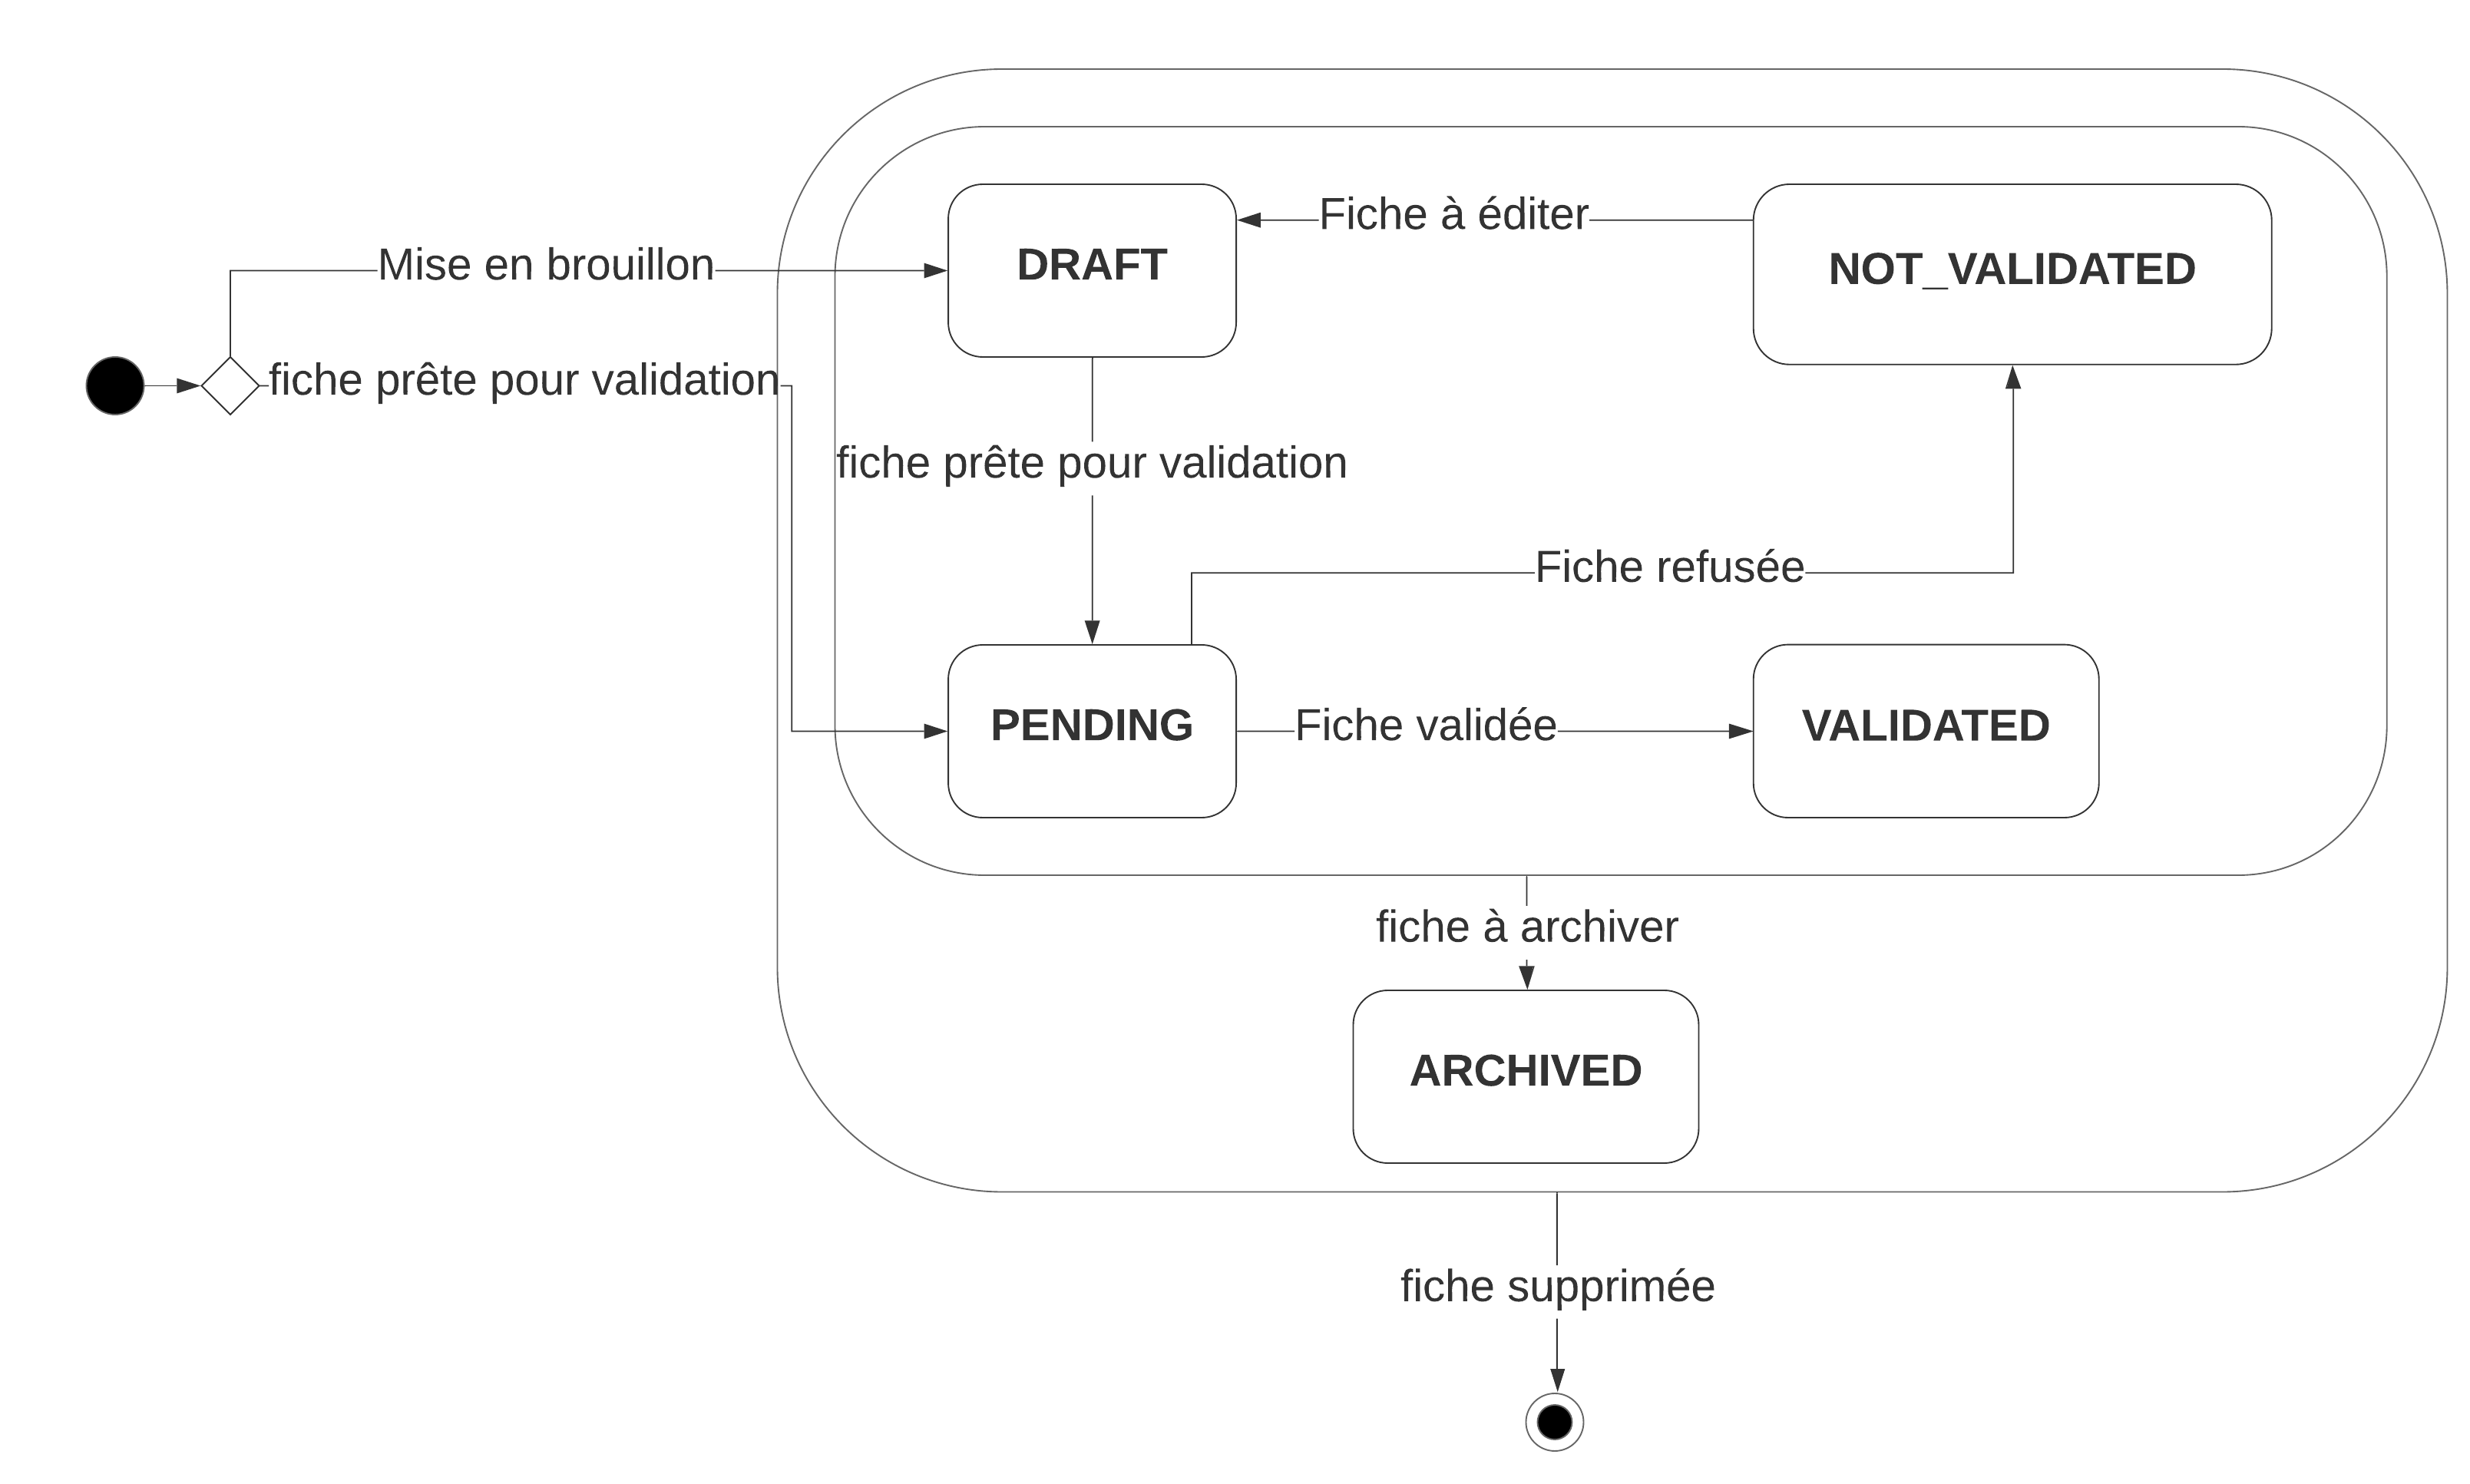
\includegraphics[width=\textwidth,height=\textheight,keepaspectratio]{images/StateFiches.png}
    \centering
    \caption{Diagramme UML à états pour l'état d'une \gls{fiche}}
    \label{pic:stateDiagramForFiches}
\end{figure}

\subsection*{État d'un \gls{tag}}

Une des questions annexes au sujet des \glspl{fiche} est la gestion des \glspl{tag}. En effet, les \glspl{tag} étant des éléments indispensables d'une \gls{fiche} de qualité pour un meilleur référencement, il convient d'établir une stratégie précise pour exploiter au mieux ceux-ci. \\

Durant notre analyse, nous avons pu constater deux écoles de pensée bien distinctes (comparable à ce qui existe en économie) : 
\begin{itemize}
    \item laissez-faire : Il s'agit de donner une liberté totale en matière de marquage (en utilisant aussi bien des \glspl{tag} existants que non). Bien que cette approche a le mérite de faire émerger de nouveaux \glspl{tag} par les contributions d'utilisateurs, cela restreint les possibilités de modération.
    \item l'interventionnisme : Il s'agit de restreindre le choix en matière de marquage (exclusivement des \glspl{tag} existants). Bien que cette approche rend la modération facile, cela restreint les possibilités de s'adapter à une réalité changeante.
\end{itemize}

Nous avons remarqué qu'aucune de ces deux possibilités ne se distinguait suffisamment de l'autre pour répondre de manière optimale à la problématique.
C'est pourquoi nous avons fait le choix d'une 3e voie, qui se situe donc entre ces 2 manières de penser. Tout comme les \glspl{fiche}, il s'agit d'associer un état à chaque \gls{tag} pour distinguer sa situation propre. Le diagramme UML à états ci-dessous représente ces états et les principales transitions entre états (pour ne pas surcharger celui-ci) :

% width=\textwidth,height=\textheight,keepaspectratio
\begin{figure}[H]
    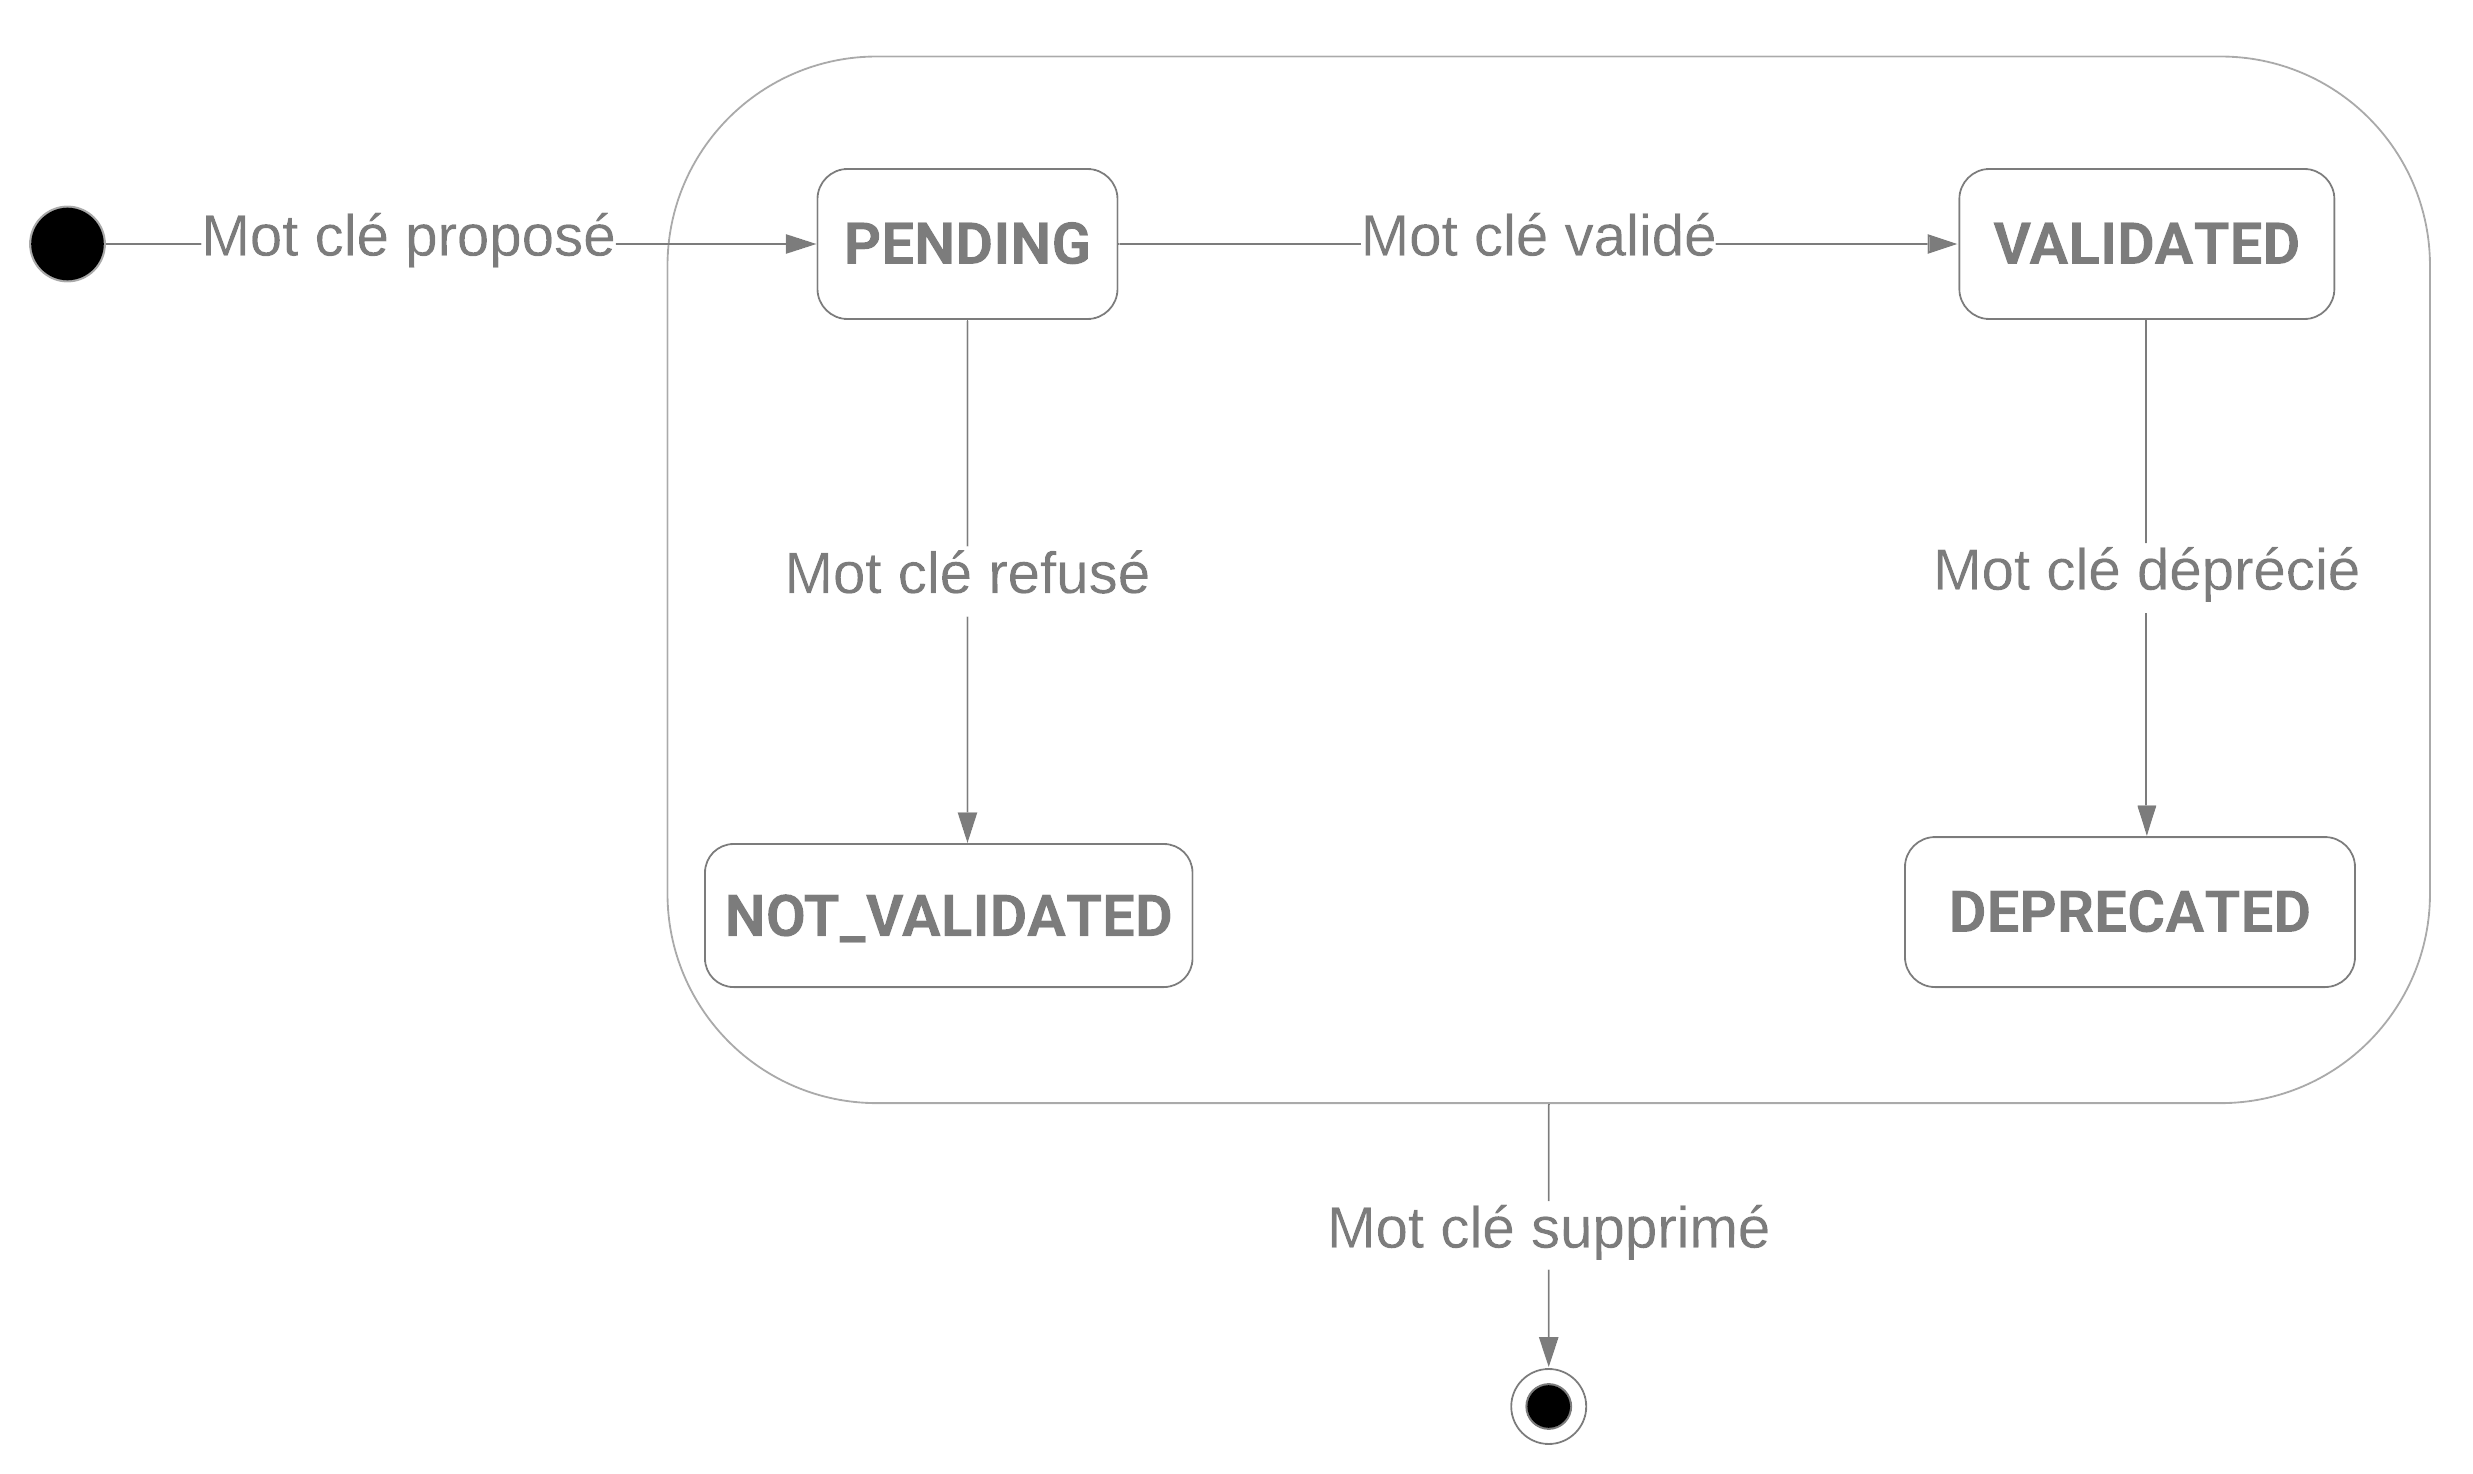
\includegraphics[width=\textwidth,height=\textheight,keepaspectratio]{images/StateTags.png}
    \centering
    \caption{Diagramme UML à états pour l'état d'un \gls{tag}}
    \label{pic:stateDiagramForTags}
\end{figure}

\subsection*{Maintenabilité aisée des données}

Lors de notre analyse, un besoin particulièrement criant s'est présenté à nous : sans être informaticien ou connaître les technologies réalisant le stockage de données, il faut disposer d'un moyen de lire/modifier ces données avec aisance. \\

Cela implique dès lors de proposer des opérations pour manipuler les différentes ressources de notre application (\glspl{fiche}, \glspl{tag}, \glspl{tagCat}, etc...). Pour compléter la panoplie, nous avons conçu un moyen d'importer / exporter les \glspl{fiche}, notamment pour répondre aux besoins d'archivage.

\pagebreak


\section{Analyse non fonctionnelle}
\label{section:AnalyseNonFonctionnelle}
% On explique ici (design, ergonomie)
% Donner les critères d'ergonomie
% Pas forcément des tonnes de page : à priori 3-4 max devraient suffire

\subsection*{Sécurité}

La sécurité d'une application doit faire l'objet d'une attention non négligeable, particulièrement dans le contexte de notre époque mouvementée dans bien des domaines. Il est donc essentiel de se poser les bonnes questions (par exemple en utilisant \Gls{QQOQCCP}). Pour relever ce défi, une méthode possible est la \textbf{AAA}\footnote{Acronyme anglophone pour "\textbf{A}uthentication/\textbf{A}uthorization/\textbf{A}ccounting", que l'on peut traduire en français par "authentification/autorisation/traçabilité" }
consistant en 3 piliers : 

\begin{description}
    \item[Authentification :] Il s'agit du fait de prouver l'utilisateur que l'on prétend être. Une manière fréquemment utilisée sur de nombreux sites consiste en association d'un nom d'utilisateur et d'un mot de passe.
    \item[Autorisation :] Il s'agit du fait de vérifier quelles ressources accessibles et les opérations (par exemple les \Gls{crud}) permises sur celles-ci pour l'utilisateur authentifié.
    \item[Traçabilité :] Il s'agit du fait d'enregistrer tous les faits et gestes des utilisateurs authentifiés. Les informations ainsi collectées permettent principalement de prévenir/comprendre des problèmes. 
\end{description}

% TODO maybe citer la section dans l'implémentation

\subsection*{Maintenance et évolution}

Ce travail s'est déroulé dans le cadre d'un mémoire universitaire. Étant donné que la problématique du mémoire ne risque pas de faiblir d'intensité dans les années à venir, une reprise/évolution du projet par une équipe ultérieure inconnue est une possibilité à ne pas exclure. Il convient donc de mettre en place les dispositions nécessaires pour faciliter la maintenance de notre application. \\

Pour cela, nous avons sélectionné des technologies relativement bien documentées et populaires de telle sorte que nos successeurs n'éprouvent pas de difficulté à se former à celles-ci. Vous pourrez retrouver des explications plus détaillées à ce sujet dans la section \ref{section:choixTechnologiques}.

\subsection*{Ergonomie}

Une application web à destination d'un public varié et conséquent se doit d'avoir une interface simple et efficace pour ne pas perdre ses utilisateurs et gagner en popularité. On pourrait considérer que le design d'une application est subjectif, mais un point à ne sûrement pas négliger se situe autour de l'ergonomie. La question à se poser pour chaque interface est alors de savoir comment disposer les éléments afin de rendre la navigation la plus claire possible. Nous nous sommes donc concentrés sur cette problématique en élaborant un patchwork que vous pouvez consulter à la fin de la section \ref{section:problem}\\

Au fur et à mesure de nos meetings avec le \textit{Pr. Kim Mens} et \textit{Olivier Goletti}, les conseils et recommandations ont souvent été pris en compte pour améliorer l'expérience utilisateur. Par la même occasion, nous avons fait tester l'application à différents utilisateurs (amis, designer) tout au long de la phase de développement afin de nous faire part de leur ressenti.

\pagebreak
\section {Contraintes}
\label{sec:ContraintesCdc}

Une première contrainte évidente est indubitablement le temps. Nous avons consacré une année académique entière sur ce mémoire, mais ce n'est certainement pas assez pour rendre mature \texttt{SourceCode}.\\

Pour la partie \gls{frontend}, nous avons décidé de nous consacrer uniquement sur le design et l'ergonomie d'un desktop ayant une largeur minimale de 1550 pixels. Pour l'instant, nous avons recommandé aux utilisateurs de l'application ayant une petite résolution de modifier l'échelle du navigateur internet afin d'avoir une expérience optimale malgré notre contrainte. Créer les autres déclinaisons pour petits desktop, tablettes et smartphones ne nous auraient pas permis d'intégrer toutes les fonctionnalités qu'on avait prévu d'ajouter sur la plateforme, car cela aurait pris trop de temps (modifier la disposition des éléments, créer de nouveaux éléments, changer le layout, ...). \\

Pour la partie \gls{backend}, il nous a été imposé de travailler avec une base de données relationnelle\footnote{
    \href{https://fr.wikipedia.org/wiki/Base\_de\_donn\%C3\%A9es\_relationnelle}
    {https://fr.wikipedia.org/wiki/Base\_de\_données\_relationnelle}
} dont PostgreSQL\footnote{
    \url{https://www.postgresql.org/}
} a été le système de gestion imposé. Ce type de base de données dispose de propriétés très intéressantes dont notamment les \textbf{ACID}\footnote{
    \href{https://fr.wikipedia.org/wiki/Propri\%C3\%A9t\%C3\%A9s\_ACID}
    {https://fr.wikipedia.org/wiki/Propriétés\_ACID}
}, que vous retrouvez sur la figure \ref{pic:ACIDproperties} (par souci de clarté, l'abréviation \textbf{MAJ} désigne le terme "mise(s) à jour") :

\begin{figure}[H]
    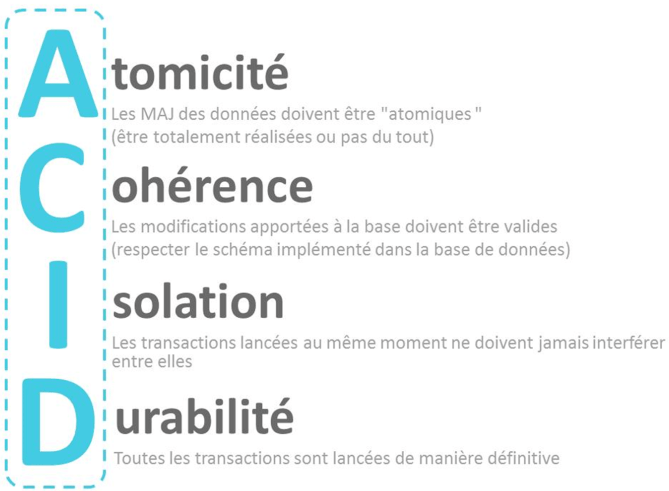
\includegraphics[width=\textwidth,height=\textheight,keepaspectratio]{images/ACID.png}
    \centering
    \caption[Propriétés \textbf{ACID}]{Propriétés \textbf{ACID} \cite{bigdata_cap}}
    \label{pic:ACIDproperties}
\end{figure}

\pagebreak

Étant donné que ces propriétés sont assez contraignantes, le lecteur attentif (ou lectrice attentive) que vous êtes est en droit de remettre en question cette contrainte technique et il est donc utile de recourir au théorème \textbf{CAP} pour la justifier.
Comme expliqué par un article \cite{acid_cap}, chaque lettre de cette anagramme représente une certaine propriété :
\begin{description}
    \item[\textbf{C}onsistency (Cohérence) :] "Une donnée n'a qu'un seul état visible, quel que soit le nombre de réplicas"
    \item[\textbf{A}vailability (Disponibilité) :] "Tant que le système tourne (distribué ou non), la donnée doit être disponible"
    \item[\textbf{P}artition Tolerance (Distribution) :] "Quel que soit le nombre de serveurs, toute requête doit fournir un résultat correct" 
\end{description}

Comme souligné dans ce même article \cite{acid_cap}, le théorème dit que "dans toute base de données, vous ne pouvez respecter au plus que 2 propriétés".
Grâce à ce théorème, nous pouvons mieux justifier l'obligation de PostgreSQL par rapport à des solutions alternatives, comme le montre la figure \ref{pic:capTriangleWithSomeDatabases} :

\begin{figure}[H]
    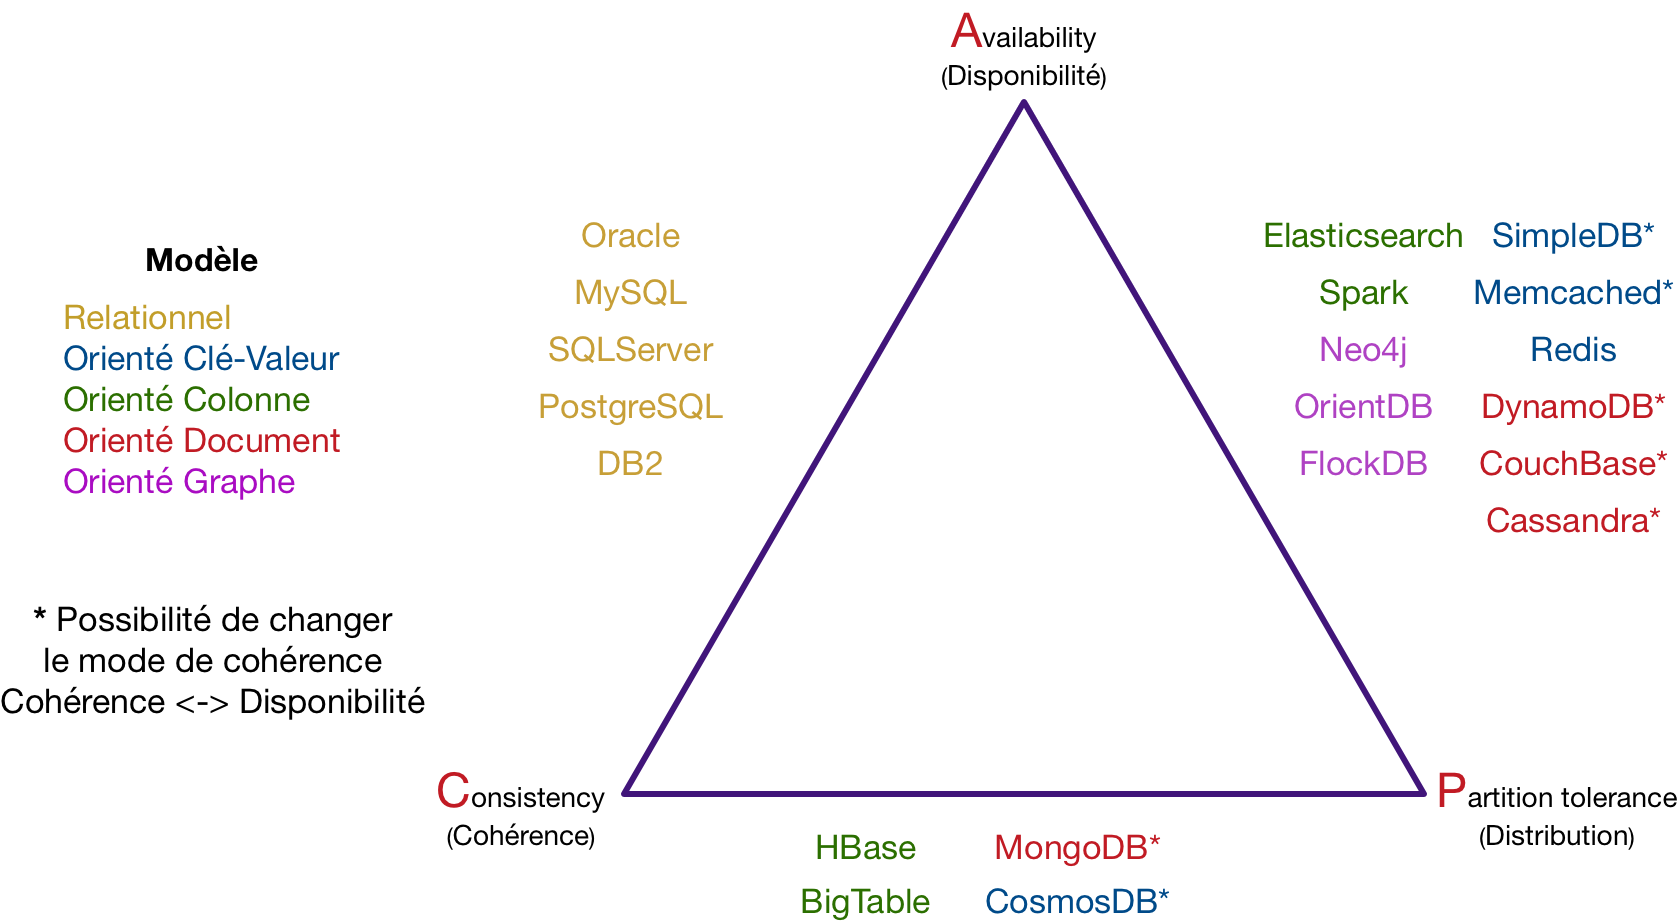
\includegraphics[width=\textwidth,height=\textheight,keepaspectratio]{images/triangleCAP_with_databases.png}
    \centering
    \caption[Triangle \textbf{CAP} avec quelques bases de données]{Triangle \textbf{CAP} avec quelques bases de données \cite{acid_cap}}
    \label{pic:capTriangleWithSomeDatabases}
\end{figure}